\de{ĐỀ THI HỌC KỲ II NĂM HỌC 2022-2023}{THPT Nguyễn Chí Thanh}


\begin{bt}%[0T7B2-1]%[0T7B3-2]%[Dự án đề kiểm tra HKII NH22-23- Nguyễn Tú]%[THPT Nguyễn Chí Thanh]%
	\begin{enumerate}
		\item Giải bất phương trình sau: $x^2 - 5x - 6 \geq 0$
		\item Giải phương trình sau: $\sqrt{3 x^2-9 x-5}+2 x=5$
	\end{enumerate}
\loigiai{
\begin{enumerate}
	\item {Giải bất phương trình sau: $x^2 - 5x - 6 \geq 0$.\\
	Phương trình $x^2 - 5x - 6 = 0$ có 
	\begin{itemize}
		\item $a>0$.
		\item $\Delta = 49 > 0$.
		\item $f(x)=0$ có hai nghiệm là $\hoac{&x=6\\&x=-1.}$
	\end{itemize}
	Ta có bảng xét dấu sau: 
	\begin{center}
		
\begin{tikzpicture}
			\tkzTabInit
			[lgt=3.5,espcl=2] % tùy chọn
			{$x$/0.8, $x^2 - 5x - 6$/1 }
			{$-\infty$, $-1$, $6$,$+\infty$}
			\tkzTabLine{,+,z,-,z,+,}
		\end{tikzpicture}
	\end{center}
	Do đó nghiệm của bất phương trình $x^2 - 5x - 6 \geq 0$ là $x \in (-\infty;-1)\cup (6;+\infty)$}
	\item {Giải phương trình sau: $\sqrt{3x^2-9x-5}+2x=5$
	\allowdisplaybreaks
	\begin{eqnarray*}
		&& \sqrt{3x^2-9x-5}=5-2x \quad \hfil(1)\\
		&\Leftrightarrow& 3x^2-9x-5=(5-2x)^2=25-20x+4x^2\\
		&\Leftrightarrow& x^2-11x+30=0\\
		&\Leftrightarrow& \hoac{&x=5\\&x=6.}
	\end{eqnarray*}
	Thử lại vào phương trình (1) ta thấy các giá trị $x=5$, $x=6$ thỏa mãn.\\
	Nên nghiệm của phương trình $\sqrt{3x^2-9x-5}+2 x=5$ là $x=5$, $x=6$.}
\end{enumerate}
}
\end{bt}
%Câu 2
\begin{bt}%[0T9B2-2]%[0T9B4-1]%[Dự án đề kiểm tra HKII NH22-23- Nguyễn Tú]%[THPT Nguyễn Chí Thanh]%
	\begin{enumerate}
		\item Viết phương trình tham số và phương trình tổng quát của đường thằng $d$ đi qua điểm $A(5 ; 4)$ và có vectơ chỉ phương $\vec{u}=(1 ; 3)$.
		\item Gọi tên, tìm tọa độ tiêu điểm, tọa độ các đỉnh của đường conic sau: $(C): \dfrac{x^2}{169}+\dfrac{y^2}{25}=1$
	\end{enumerate}
	\loigiai{
		\begin{enumerate}
		\item {\textit{Phương trình tổng quát đường thẳng $d$ đi qua điểm $A (5 ; 4)$ và có vectơ pháp tuyến $\vec{u}=(3 ; -1)$.}
		\allowdisplaybreaks
		\begin{eqnarray*}
			& & d \colon  3(x-5)+-1(y-4)=0\\
			&\Leftrightarrow& 3x-y-11=0.
		\end{eqnarray*}
		\textit{Phương trình tham số đường thẳng $d$ đi qua điểm $A (5 ; 4)$ và có vectơ chỉ phương $\vec{u}=(1 ; 3)$.}
		\begin{eqnarray*}
			d \colon \heva{&x=5+t \\&y=4+3t.}
		\end{eqnarray*}		
		}
		\item Vì $(C)$ có dạng $\dfrac{x^2}{a^2}+\dfrac{y^2}{b^2}=1$ nên $(C)$ là Elip với $\heva{&a=13\\&b=5}$ 
		$(C)$ cắt trục hoành tại $A_1 (-13;0)$ và $A_2 (13;0)$.\\
		$(C)$ cắt trục trung tại $B_1 (0;-5)$ và $B_2 (0;5)$.\\
		$\Rightarrow c=\sqrt{a^2-b^2}=12$, do đó tọa độ tiêu điểm là $F_1 (-12;0)$ và $F_2 (12;0)$.
	\end{enumerate}	
	}
\end{bt}
%Câu 3
\begin{bt}%[0T8B3-1]%[0T0B2-2]%[Dự án đề kiểm tra HKII NH22-23- Nguyễn Tú]%[THPT Nguyễn Chí Thanh]%
	Lời dẫn
	\begin{enumerate}
		\item Khai triển và rút gọn biểu thức: $A=(1+x)^5+(1-x)^5$.
		\item Gieo $2$ con xúc xắc cân đối và đồng chất, tính xác suất của biến cố $A$  \lq \lq Tổng số chấm xuất hiện trên hai mặt của xúc xắc bằng $7$ \rq \rq?
	\end{enumerate}
	\loigiai{
	\begin{enumerate}
		\item {Khai triển và rút gọn biểu thức: $A=(1+x)^5+(1-x)^5$.\\
		Ta có: $\heva{&(1+x)^5=1+5x+10x^2+10x^3+5x^4+x^5\\ &(1-x)^5=1-5x+10x^2-10x^3+5x^4-x^5.}$\\
		Do đó: $A=(1+x)^5+(1-x)^5 = 2+20x^2+10x^4$.
		}
		\item {Không gian mẫu $n(\Omega)=6^2=36$,\\
	 	Biến cố $A \colon$ \lq \lq Tổng số chấm xuất hiện trên hai mặt của xúc xắc bằng $7$ \rq \rq.\\
	 	Các trường hợp thỏa biến cố $A$ là $(1,6)$, $(6,1)$, $(5,2)$, $(2,5)$, $(4,3)$, $(3,4)$.\\
	 	Do đó $n(A)=6$.\\
	 	Xác suất \lq \lq Tổng số chấm xuất hiện trên hai mặt của xúc xắc bằng $7$ \rq \rq là:\\
	 	$P(A)=\dfrac{n(A)}{n(\Omega)}=\dfrac{6}{36}=\dfrac{1}{6}$
		}
	\end{enumerate}	
	}
\end{bt}
%Câu 4
\begin{bt}%[0T9B3-3]%[Dự án đề kiểm tra HKII NH22-23- Nguyễn Tú]%[THPT Nguyễn Chí Thanh]%
	Cho đường tròn $(C)$ có phương trình $x^2+y^2-6x-2y-15=0$. Viết phương trình tiếp tuyến với $(C)$ song song với đường thẳng $8 x+6y+99=0$.
	\loigiai{
	Gọi $\Delta$ là tiếp tuyến của đường tròn $(C)$.\\
	Do $\Delta$ song song với đường thẳng $8x+6y+99=0$ nên phương trình đường thẳng $\Delta$ có dạng $8x+6y+c=0$ $(c \ne 99)$.\\
	Phương trình đường tròn $(C): x^2+y^2-6x-2y-15=0$ có tâm $I(3;1)$ và bán kính $R=5$.\\
	\begin{eqnarray*}
		\text{Ta có} d(I,\Delta)=R=5 &=&\dfrac{|8\cdot3 + 6\cdot1 +c|}{\sqrt{8^2 +6^2}}.\\
		&\Leftrightarrow& |30 +c| = 50 \Leftrightarrow \hoac{&30+c=50 \\ &30+c=-50} 
		\Leftrightarrow \hoac{&c=20 \\ &c=-80.}\\
	\end{eqnarray*}	
	Vậy phương trình tiếp tuyến của đường tròn $(C) \colon x^2+y^2-6x-2y-15=0$ là $\Delta_1 \colon 8x+6y+20=0$ hoặc $\Delta_2 \colon 8x+6y-80=0 $
	}
\end{bt}

\begin{bt}%[0D9BP-3]%[Dự án đề kiểm tra HKII NH22-23- Huỳnh Quy]%[THPT Nguyễn Chí Thanh-Tp.HCM]
	Trên một giá sách có các quyển sách về bốn môn học là \textit{Toán}, \textit{Vật lý}, \textit{Hóa học} và \textit{Sinh học} bao gồm $7$ quyển sách Toán, $6$ quyển sách Vật lý, $5$ quyển sách Hóa học, $4$ quyển sách Sinh học. Lấy ngẫu nhiên ra $4$ quyển sách. Tính xác suất của biến cố $A$: ``Trong $4$ quyển sách lấy ra có đúng hai môn học và số lượng bằng nhau''. 
	\loigiai{
	Số phần tử của không gian mẫu là $n(\Omega)=\mathrm{C}_{22}^{4}=7315$.\\
	Gọi $A$ là biến cố: ``Trong $4$ quyển sách lấy ra có đúng hai môn học và số lượng bằng nhau''. \\
	Ta có $n(A)=\mathrm{C}_{7}^{2}\cdot \mathrm{C}_{6}^{2}+\mathrm{C}_{7}^{2}\cdot \mathrm{C}_{5}^{2}+\mathrm{C}_{7}^{2}\cdot \mathrm{C}_{4}^{2}+\mathrm{C}_{6}^{2}\cdot \mathrm{C}_{5}^{2}+\mathrm{C}_{6}^{2}\cdot \mathrm{C}_{4}^{2}+\mathrm{C}_{5}^{2}\cdot \mathrm{C}_{4}^{2}=951$.\\	
	Xác suất cần tìm là $P(A)=\dfrac{n(A)}{n(\Omega)}=\dfrac{951}{7315}$.}
\end{bt}

\begin{bt}%[0D6KH-2]%[Dự án đề kiểm tra HKII NH22-23- Huỳnh Quy]%[THPT Nguyễn Chí Thanh-Tp.HCM]
	Một mảnh vườn trồng hoa có hình dạng là một tam giác vuông. Biết tam giác vuông này có độ dài của hai cạnh góc vuông hơn kém là $70$m và chu vi của tam giác vuông này bằng $300$m. Hãy tính diện tích của mảnh vườn trồng hoa đó.
	\loigiai{
	Gọi $x$ (m) là độ dài một cạnh góc vuông của mảnh vườn ($x>0$). \\
	Độ dài cạnh góc vuông còn lại là $x+70$ (m).\\
	Độ dài cạnh huyền là $\sqrt{x^2+(x+70)^2}$ (m).\\
	Chu vi tam giác là 
	\begin{eqnarray*}
		&&x+(x+70)+\sqrt{x^2+(x+70)^2}=300\\
		&\Leftrightarrow&2x+70+\sqrt{x^2+x^2+140x+4900}=300\\
		&\Leftrightarrow&\sqrt{2x^2+140x+4900}=230-2x.\quad(*)
	\end{eqnarray*}
Bình phương hai vế phương trình $(*)$ ta được:
	\begin{eqnarray*}
		&&2x^2+140x+4900=(230-2x)^2\\
		&\Rightarrow&2x^2+140x+4900=52900-920x+4x^2\\
		&\Rightarrow&-2x^2+1060x-48000=0\\
		&\Rightarrow&\hoac{&x=480\\&x=50.}
	\end{eqnarray*}
Thử lại, ta thay các giá trị $x=480$, $x=50$ vào phương trình $(*)$, ta thấy chỉ có giá trị $x=50$ thỏa mãn.\\
Vậy phương trình $(*)$ có nghiệm $x=50$.\\
Suy ra độ dài cạnh còn lại là $x+70=120$ (m).\\
Diện tích mảnh vườn là $S=\dfrac{1}{2}\cdot 50\cdot 120=3000$ ($\mathrm{m}^{2}$).
	}
\end{bt}

\begin{bt}%[0H7KL-0]%[Dự án đề kiểm tra HKII NH22-23- Huỳnh Quy]%[THPT Nguyễn Chí Thanh-Tp.HCM]
	Dọc theo bờ biển, người ta thiết lập hệ thống định vị vô tuyến dẫn đường tầm xa để truyền tín hiệu cho máy bay hoặc tàu thủy hoạt động trên biển. Trong hệ thống đó có hai đài vô tuyến đặt lần lượt tại địa điểm $A$ và địa điểm $B$, khoảng cách $AB=650$km. Giả sử có một con tàu chuyển động trên biển với quỹ đạo nằm trên một nhánh Hypebol nhận $A$ và $B$ là hai tiêu điểm như hình. Khi đang ở vị trí $P$, máy thu tín hiệu trên con tàu chuyển đổi chênh lệch thời gian nhận các tín hiệu từ $A$ và $B$ thành hiệu khoảng cách $|PA-PB|$. Giả sử thời gian con tàu nhận được tín hiệu từ $B$ trước khi nhận được tín hiệu từ $A$ là $0{,}0012$s. Vận tốc di chuyển của tín hiệu là $3.10^{8}$m/s. Lập phương trình hypebol mô tả quỹ đạo chuyển động của con tàu.
	\begin{center}
		\definecolor{lightcornflowerblue}{rgb}{0.6, 0.81, 0.93}
		\definecolor{cerulean}{rgb}{0.0, 0.48, 0.65}
		\definecolor{chamoisee}{rgb}{0.63, 0.47, 0.35}
		\definecolor{fashionfuchsia}{rgb}{0.96, 0.0, 0.63}
		\definecolor{grannysmithapple}{rgb}{0.66, 0.89, 0.63}
		\definecolor{fawn}{rgb}{0.9, 0.67, 0.44}
		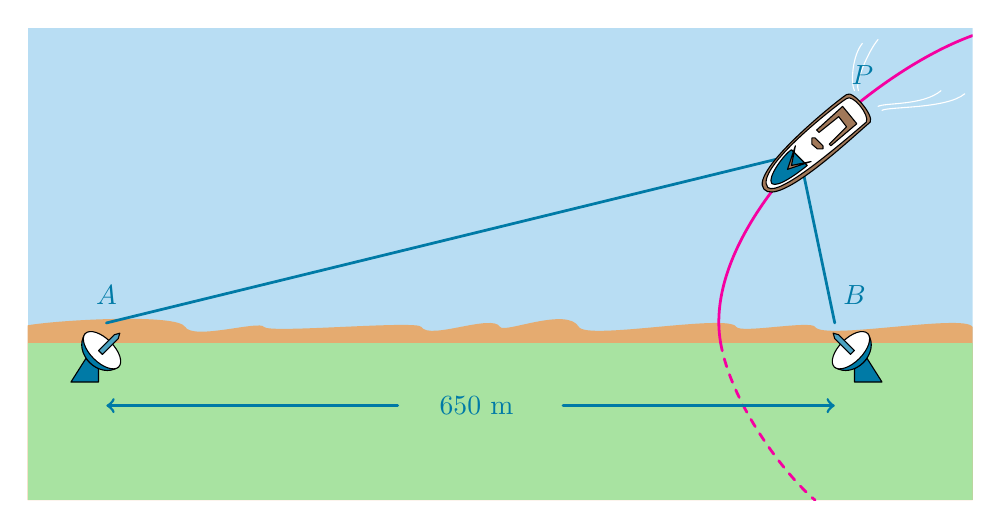
\begin{tikzpicture}[line join=round, line cap=round,scale=1,transform shape]
			\clip (-6,-3) rectangle (6,3);
			
			\fill[lightcornflowerblue!70] (-6,-3) rectangle (6,3);
			\fill[fawn,line width=1](-6,-.78)
			..controls +(10:.4) and +(120:.2) ..(-4,-.8)
			..controls +(-60:.2) and +(120:.1) ..(-3,-.8)
			..controls +(-60:.1) and +(120:.1) ..(-1,-.8)
			..controls +(-60:.2) and +(120:.2) ..(0,-.8)
			..controls +(-60:.1) and +(120:.3) ..(1,-.8)
			..controls +(-60:.2) and +(120:.2) ..(3,-.8)
			..controls +(-60:.1) and +(120:.1) ..(4,-.8)
			..controls +(-60:.2) and +(120:.2) ..(6,-.8)--(6,-3)--(-6,-3)--cycle;
			
			\fill[grannysmithapple] (-6,-3) rectangle (6,-1);
			
			\draw[fashionfuchsia,line width=1](6,2.9)
			..controls +(-160:1.5) and +(100:1.5) ..(2.8,-1);
			\draw[dashed,fashionfuchsia,line width=1](2.8,-1)
			..controls +(-80:.8) and +(140:.5) ..(4,-3);
			
			\tikzset{tram_phat/.pic={
					\def\T{ 
						(-5.26,-1.2)--(-5.45,-1.5)--(-5.1,-1.5)--(-5.1,-1.33)..controls +(150:.1) and +(-50:.1) ..cycle;
					}
					\fill[cerulean] \T;
					\draw\T;
					\draw[fill=cerulean,rotate=-45](-3.1,-4.35)
					..controls +(-80:.3) and +(-100:.3) ..(-2.5,-4.35);
					\draw[fill=white,rotate=-45](-2.5,-4.35) arc (0:360:.3 cm and .15cm);
					\draw[fill=cerulean!70](-5.1,-1.1)--(-4.9,-.9)--(-4.83,-.88)--(-4.85,-.95)--(-5.05,-1.15)--cycle;
			}}
			\tikzset{tau/.pic={
					\def\Ta1{ 
						(4.4,2.15)
						..controls +(-150:.1) and +(130:.3) ..(3.35,.95)
						..controls +(-50:.3) and +(-140:.3) ..(4.7,1.8)
						..controls +(60:.1) and +(40:.1) ..cycle
						;
					}
					\fill[chamoisee] \Ta1;
					\draw\Ta1;
					\def\Ta2{ 
						(4.4,2.1)
						..controls +(-150:.1) and +(130:.3) ..(3.4,.97)
						..controls +(-40:.2) and +(-140:.3) ..(4.65,1.8)
						..controls +(60:.1) and +(40:.1) ..cycle
						;
					}
					\fill[white] \Ta2;
					\draw\Ta2;
					
					\def\Ta3{ 
						(3.7,1.45)
						..controls +(-150:.1) and +(130:.1) ..(3.45,1.02)
						..controls +(-40:.1) and +(-140:.1) ..(3.9,1.25)--cycle
						;
						
					}
					\fill[cerulean] \Ta3;
					\draw\Ta3;
					
					\def\Ta4{ 
						(3.75,1.5)--(3.7,1.25)--(3.95,1.3)--(3.65,1.2)--cycle
						(3.96,1.6)--(4,1.6)--(4.1,1.5)--(4.1,1.46)--(4.03,1.46)--(3.96,1.52)--cycle
						(4.35,2)--(4.53,1.78)--(4.2,1.5)--(4.18,1.52)--(4.4,1.74)--(4.3,1.87)--(4.05,1.67)--(4.02,1.7)--cycle;
					}
					\fill[chamoisee] \Ta4;
					\draw\Ta4;
					
			}}
			\draw[cerulean,line width=1] (-5,-.75)--(3.8,1.4)--(4.25,-.75);
			\draw[cerulean,line width=1,<-] (-5,-1.8)--(-1.3,-1.8);
			\draw[cerulean,line width=1,->] (.8,-1.8)--(4.25,-1.8);
			\path
			(0,0)pic[scale=1]{tram_phat}
			(-.6,0)pic[scale=1,rotate=180,yscale=-1]{tram_phat}
			(0,0)pic[scale=1]{tau};
			\node[cerulean] at (-5,-.4) {$A$};
			\node[cerulean] at (-.3,-1.8) {$650$ m};
			\node[cerulean] at (4.5,-.4) {$B$};	
			
			\draw[white] 
			(4.8,2)
			..controls +(30:.1) and +(-140:.3) ..(5.6,2.2)
			(4.85,1.95)
			..controls +(30:.1) and +(-140:.3) ..(5.9,2.16)
			(4.5,2.2)
			..controls +(120:.1) and +(-130:.2) ..(4.6,2.8)
			(4.55,2.2)
			..controls +(120:.1) and +(-130:.2) ..(4.8,2.85)
			;
			
			\node[cerulean] at (4.6,2.4) {$P$};
		\end{tikzpicture}
	\end{center}
\loigiai{
	Phương trình hypebol có dạng: $\dfrac{x^2}{a^2}-\dfrac{y^2}{b^2}=1$ ($a>0$, $b>0$).\\
	Theo đề, tiêu cự $AB=650$ (km) $\Leftrightarrow 2c=650\Leftrightarrow c=325$.\\
	Lại có $|PA-PB|=2a=3\cdot 10^{8}\cdot 0{,}0012=360000\,(\mathrm{m})=360\,(\mathrm{km})\Leftrightarrow a=180\,(\mathrm{km})$.\\
	Mà $c^2=a^2+b^2\Rightarrow b^2=c^2-a^2=325^2-180^2=73225$.\\
	Vậy phương trình hypebol cần tìm là:
	\[
	\dfrac{x^2}{180^2}-\dfrac{y^2}{73225}=1\Leftrightarrow \boxed{\dfrac{x^2}{32400}-\dfrac{y^2}{73225}=1}.
	\]
}
\end{bt}